\documentclass{standalone}
\usepackage{tikz}
\usetikzlibrary{patterns, positioning}

\begin{document}
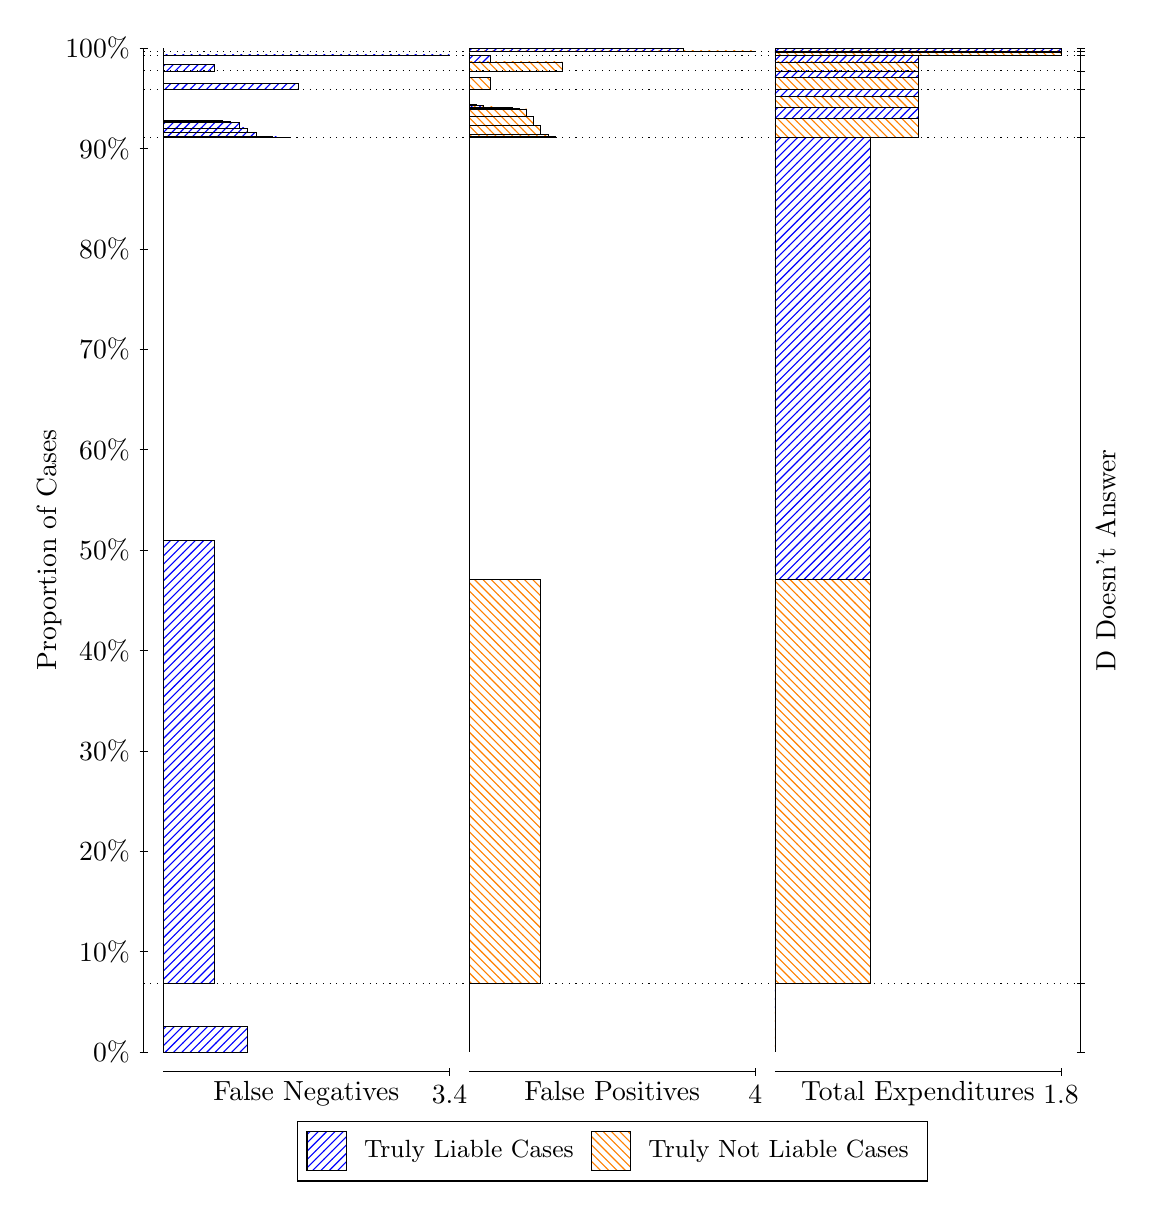
\begin{tikzpicture}
\draw[black, very thin] (1.5,1.75) -- (1.5,14.5);
\node[rotate=90, anchor=center] at (0.3, 8.125) {Proportion of Cases};
\draw[black, very thin] (1.45,1.75) -- (1.55,1.75);
\node[anchor=east] at (1.45, 1.75) {0\%};
\draw[black, very thin] (1.45,3.025) -- (1.55,3.025);
\node[anchor=east] at (1.45, 3.025) {10\%};
\draw[black, very thin] (1.45,4.3) -- (1.55,4.3);
\node[anchor=east] at (1.45, 4.3) {20\%};
\draw[black, very thin] (1.45,5.575) -- (1.55,5.575);
\node[anchor=east] at (1.45, 5.575) {30\%};
\draw[black, very thin] (1.45,6.85) -- (1.55,6.85);
\node[anchor=east] at (1.45, 6.85) {40\%};
\draw[black, very thin] (1.45,8.125) -- (1.55,8.125);
\node[anchor=east] at (1.45, 8.125) {50\%};
\draw[black, very thin] (1.45,9.4) -- (1.55,9.4);
\node[anchor=east] at (1.45, 9.4) {60\%};
\draw[black, very thin] (1.45,10.675) -- (1.55,10.675);
\node[anchor=east] at (1.45, 10.675) {70\%};
\draw[black, very thin] (1.45,11.95) -- (1.55,11.95);
\node[anchor=east] at (1.45, 11.95) {80\%};
\draw[black, very thin] (1.45,13.225) -- (1.55,13.225);
\node[anchor=east] at (1.45, 13.225) {90\%};
\draw[black, very thin] (1.45,14.5) -- (1.55,14.5);
\node[anchor=east] at (1.45, 14.5) {100\%};

\draw[black, very thin] (13.4,1.75) -- (13.4,14.5);
\draw[black, very thin] (13.35,1.75) -- (13.45,1.75);
\node[anchor=west] at (13.35, 1.75) {};
\draw[black, very thin] (13.35,2.6233) -- (13.45,2.6233);
\node[anchor=west] at (13.35, 2.6233) {};
\draw[black, very thin] (13.35,13.367) -- (13.45,13.367);
\node[anchor=west] at (13.35, 13.367) {};
\draw[black, very thin] (13.35,13.97) -- (13.45,13.97);
\node[anchor=west] at (13.35, 13.97) {};
\draw[black, very thin] (13.35,14.209) -- (13.45,14.209);
\node[anchor=west] at (13.35, 14.209) {};
\draw[black, very thin] (13.35,14.404) -- (13.45,14.404);
\node[anchor=west] at (13.35, 14.404) {};
\draw[black, very thin] (13.35,14.454) -- (13.45,14.454);
\node[anchor=west] at (13.35, 14.454) {};
\draw[black, very thin] (13.35,14.5) -- (13.45,14.5);
\node[anchor=west] at (13.35, 14.5) {};

\draw[black, very thin, pattern color=blue, pattern=north east lines] (1.75,1.75) rectangle (2.8186,2.0773);
\draw[black, very thin, pattern color=orange, pattern=north west lines] (1.75,2.0773) rectangle (1.75,2.6233);
\draw[black, very thin, pattern color=blue, pattern=north east lines] (1.75,2.6233) rectangle (2.3912,8.2424);
\draw[black, very thin, pattern color=orange, pattern=north west lines] (1.75,8.2424) rectangle (1.75,13.367);
\draw[black, very thin, pattern color=blue, pattern=north east lines] (1.75,13.367) rectangle (3.3529,13.369);
\draw[black, very thin, pattern color=blue, pattern=north east lines] (1.75,13.369) rectangle (3.2461,13.371);
\draw[black, very thin, pattern color=blue, pattern=north east lines] (1.75,13.371) rectangle (3.1392,13.376);
\draw[black, very thin, pattern color=blue, pattern=north east lines] (1.75,13.376) rectangle (3.0324,13.382);
\draw[black, very thin, pattern color=blue, pattern=north east lines] (1.75,13.382) rectangle (2.9255,13.433);
\draw[black, very thin, pattern color=blue, pattern=north east lines] (1.75,13.433) rectangle (2.8186,13.487);
\draw[black, very thin, pattern color=blue, pattern=north east lines] (1.75,13.487) rectangle (2.7118,13.551);
\draw[black, very thin, pattern color=blue, pattern=north east lines] (1.75,13.551) rectangle (2.6049,13.57);
\draw[black, very thin, pattern color=blue, pattern=north east lines] (1.75,13.57) rectangle (2.498,13.585);
\draw[black, very thin, pattern color=orange, pattern=north west lines] (1.75,13.585) rectangle (1.75,13.97);
\draw[black, very thin, pattern color=blue, pattern=north east lines] (1.75,13.97) rectangle (3.4598,14.054);
\draw[black, very thin, pattern color=orange, pattern=north west lines] (1.75,14.054) rectangle (1.75,14.209);
\draw[black, very thin, pattern color=blue, pattern=north east lines] (1.75,14.209) rectangle (2.3912,14.29);
\draw[black, very thin, pattern color=orange, pattern=north west lines] (1.75,14.29) rectangle (1.75,14.404);
\draw[black, very thin, pattern color=blue, pattern=north east lines] (1.75,14.404) rectangle (5.3833,14.413);
\draw[black, very thin, pattern color=orange, pattern=north west lines] (1.75,14.413) rectangle (1.75,14.454);
\draw[black, very thin, pattern color=orange, pattern=north west lines] (1.75,14.454) rectangle (1.75,14.463);
\draw[black, very thin, pattern color=blue, pattern=north east lines] (1.75,14.463) rectangle (1.75,14.5);
\draw[black, very thin, pattern color=orange, pattern=north west lines] (5.6333,1.75) rectangle (5.6333,2.2961);
\draw[black, very thin, pattern color=blue, pattern=north east lines] (5.6333,2.2961) rectangle (5.6333,2.6233);
\draw[black, very thin, pattern color=orange, pattern=north west lines] (5.6333,2.6233) rectangle (6.5417,7.7476);
\draw[black, very thin, pattern color=blue, pattern=north east lines] (5.6333,7.7476) rectangle (5.6333,13.367);
\draw[black, very thin, pattern color=orange, pattern=north west lines] (5.6333,13.367) rectangle (6.7233,13.382);
\draw[black, very thin, pattern color=orange, pattern=north west lines] (5.6333,13.382) rectangle (6.6325,13.408);
\draw[black, very thin, pattern color=orange, pattern=north west lines] (5.6333,13.408) rectangle (6.5417,13.521);
\draw[black, very thin, pattern color=orange, pattern=north west lines] (5.6333,13.521) rectangle (6.4508,13.63);
\draw[black, very thin, pattern color=orange, pattern=north west lines] (5.6333,13.63) rectangle (6.36,13.727);
\draw[black, very thin, pattern color=orange, pattern=north west lines] (5.6333,13.727) rectangle (6.2692,13.736);
\draw[black, very thin, pattern color=orange, pattern=north west lines] (5.6333,13.736) rectangle (6.1783,13.744);
\draw[black, very thin, pattern color=orange, pattern=north west lines] (5.6333,13.744) rectangle (6.0875,13.748);
\draw[black, very thin, pattern color=orange, pattern=north west lines] (5.6333,13.748) rectangle (5.9967,13.752);
\draw[black, very thin, pattern color=blue, pattern=north east lines] (5.6333,13.752) rectangle (5.815,13.767);
\draw[black, very thin, pattern color=blue, pattern=north east lines] (5.6333,13.767) rectangle (5.7242,13.786);
\draw[black, very thin, pattern color=blue, pattern=north east lines] (5.6333,13.786) rectangle (5.6333,13.97);
\draw[black, very thin, pattern color=orange, pattern=north west lines] (5.6333,13.97) rectangle (5.9058,14.126);
\draw[black, very thin, pattern color=blue, pattern=north east lines] (5.6333,14.126) rectangle (5.6333,14.209);
\draw[black, very thin, pattern color=orange, pattern=north west lines] (5.6333,14.209) rectangle (6.8142,14.323);
\draw[black, very thin, pattern color=blue, pattern=north east lines] (5.6333,14.323) rectangle (5.9058,14.404);
\draw[black, very thin, pattern color=orange, pattern=north west lines] (5.6333,14.404) rectangle (5.6333,14.445);
\draw[black, very thin, pattern color=blue, pattern=north east lines] (5.6333,14.445) rectangle (5.6333,14.454);
\draw[black, very thin, pattern color=orange, pattern=north west lines] (5.6333,14.454) rectangle (9.2667,14.463);
\draw[black, very thin, pattern color=blue, pattern=north east lines] (5.6333,14.463) rectangle (8.3583,14.5);
\draw[black, very thin, pattern color=orange, pattern=north west lines] (9.5167,1.75) rectangle (9.5167,2.2961);
\draw[black, very thin, pattern color=blue, pattern=north east lines] (9.5167,2.2961) rectangle (9.5167,2.6233);
\draw[black, very thin, pattern color=orange, pattern=north west lines] (9.5167,2.6233) rectangle (10.728,7.7476);
\draw[black, very thin, pattern color=blue, pattern=north east lines] (9.5167,7.7476) rectangle (10.728,13.367);
\draw[black, very thin, pattern color=orange, pattern=north west lines] (9.5167,13.367) rectangle (11.333,13.606);
\draw[black, very thin, pattern color=blue, pattern=north east lines] (9.5167,13.606) rectangle (11.333,13.742);
\draw[black, very thin, pattern color=orange, pattern=north west lines] (9.5167,13.742) rectangle (11.333,13.888);
\draw[black, very thin, pattern color=blue, pattern=north east lines] (9.5167,13.888) rectangle (11.333,13.97);
\draw[black, very thin, pattern color=orange, pattern=north west lines] (9.5167,13.97) rectangle (11.333,14.126);
\draw[black, very thin, pattern color=blue, pattern=north east lines] (9.5167,14.126) rectangle (11.333,14.209);
\draw[black, very thin, pattern color=orange, pattern=north west lines] (9.5167,14.209) rectangle (11.333,14.323);
\draw[black, very thin, pattern color=blue, pattern=north east lines] (9.5167,14.323) rectangle (11.333,14.404);
\draw[black, very thin, pattern color=orange, pattern=north west lines] (9.5167,14.404) rectangle (13.15,14.445);
\draw[black, very thin, pattern color=blue, pattern=north east lines] (9.5167,14.445) rectangle (13.15,14.454);
\draw[black, very thin, pattern color=orange, pattern=north west lines] (9.5167,14.454) rectangle (13.15,14.463);
\draw[black, very thin, pattern color=blue, pattern=north east lines] (9.5167,14.463) rectangle (13.15,14.5);
\draw[black, dotted] (1.5,2.6233) -- (13.4,2.6233);
\draw[black, dotted] (1.5,13.367) -- (13.4,13.367);
\draw[black, dotted] (1.5,13.97) -- (13.4,13.97);
\draw[black, dotted] (1.5,14.209) -- (13.4,14.209);
\draw[black, dotted] (1.5,14.404) -- (13.4,14.404);
\draw[black, dotted] (1.5,14.454) -- (13.4,14.454);
\draw[black, very thin] (1.75,1.5) -- (5.3833,1.5);
\node[anchor=north] at (3.5667, 1.5) {False Negatives};
\draw[black, very thin] (5.3833,1.45) -- (5.3833,1.55);
\node[anchor=north] at (5.3833, 1.45) {3.4};

\draw[black, very thin] (5.6333,1.5) -- (9.2667,1.5);
\node[anchor=north] at (7.45, 1.5) {False Positives};
\draw[black, very thin] (9.2667,1.45) -- (9.2667,1.55);
\node[anchor=north] at (9.2667, 1.45) {4};

\draw[black, very thin] (9.5167,1.5) -- (13.15,1.5);
\node[anchor=north] at (11.333, 1.5) {Total Expenditures};
\draw[black, very thin] (13.15,1.45) -- (13.15,1.55);
\node[anchor=north] at (13.15, 1.45) {1.8};


\node[black, centered, rotate=90] at (13.72, 7.995) {D Doesn't Answer};






\draw (7.449999999999999,1.5) node[draw=none] (baseCoordinate) {};
\begin{scope}[align=center]
        \matrix[scale=0.5, draw=black, below=0.5cm of baseCoordinate, nodes={draw}, column sep=0.1cm]{
            \node[rectangle, draw, minimum width=0.5cm, minimum height=0.5cm, pattern=north east lines, pattern color=blue] {}; &
            \node[draw=none, font=\small] (B) {Truly Liable Cases}; &
            \node[rectangle, draw, minimum width=0.5cm, minimum height=0.5cm, pattern=north west lines, pattern color=orange] {}; &
            \node[draw=none, font=\small] (B) {Truly Not Liable Cases}; \\
            };
\end{scope}

\end{tikzpicture}
\end{document}